\documentclass[aps,prb,twocolumn,superscriptaddress,10pt]{revtex4-2}
\usepackage{amsmath}
\usepackage{amssymb}
\usepackage[table]{xcolor}
\usepackage{tikz}
\usetikzlibrary{quantikz}
\usetikzlibrary{decorations.pathreplacing}
\usetikzlibrary{3d,calc}
\usetikzlibrary{shapes.geometric}
\usepackage{tcolorbox}
\usepackage{tikzpeople}

\begin{document}

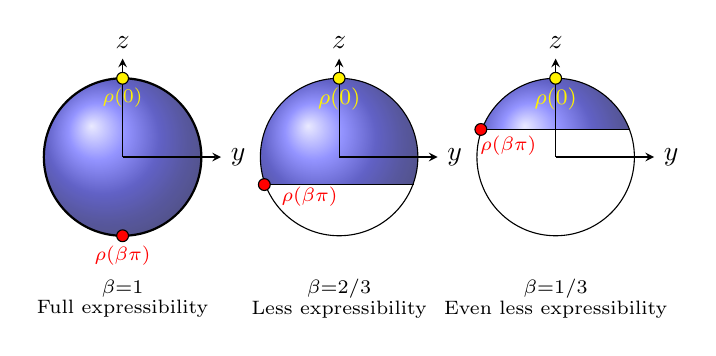
\begin{tikzpicture}
  % FIRST BLOCH SPHERE (full expressibility)
  % Draw shaded region
  \begin{scope}
    \shade[ball color=blue!75, opacity=0.75] (0,0) circle (1);
  \end{scope}
  % Axes
  \draw[-stealth] (0,0) --++ (0,1.25) node[above] {$z$};
  \draw[-stealth] (0,0) --++ (1.25,0) node[right] {$y$};
  % Equator and longitudinal lines
  \draw[thick] (1,0) arc (0:360:1);
  % Label the Bloch sphere with beta
  \node at (0,-1.8) {$\substack{\beta=1\\\textrm{Full expressibility}}$};
  \draw[fill=yellow] (0,1) circle (0.075cm) node[below] {\scriptsize\textcolor{yellow}{$\rho(0)$}};
  \draw[fill=red] (0,-1) circle (0.075cm) node[below] {\scriptsize\textcolor{red}{$\rho(\beta\pi)$}};
  % SECOND BLOCH SPHERE (0.66 expressibility)
  % Draw shaded region
  \begin{scope}
    \clip (-1+2.75,-0.35) rectangle (1+2.75,1);
    \shade[ball color=blue!75, opacity=0.75] (0+2.75,0) circle (1);
  \end{scope}
  \draw (1.8,-0.35) --++ (1.9,0);
  % Axes
  \draw[-stealth] (0+2.75,0) --++ (0,1.25) node[above] {$z$};
  \draw[-stealth] (0+2.75,0) --++ (1.25,0) node[right] {$y$};
  % Equator
  \draw (1+2.75,0) arc (0:360:1);
  % Label the Bloch sphere with beta
  \node at (0+2.75,-1.8) {$\substack{\beta=2\slash3\\\textrm{Less expressibility}}$};
  \draw[fill=yellow] (0+2.75,1) circle (0.075cm) node[below] {\footnotesize\textcolor{yellow}{$\rho(0)$}};
  \draw[fill=red] (1.8,-0.35) circle (0.075cm); 
  \node at (1.8+0.575,-0.35-0.15) {\scriptsize\textcolor{red}{$\rho(\beta\pi)$}};
  % THIRD BLOCH SPHERE (0.33 expressibility)
  % Draw shaded region
  \begin{scope}
    \clip (-1+2.75+2.75,0.35) rectangle (1+2.75+2.75,1);
    \shade[ball color=blue!75, opacity=0.75] (0+2.75+2.75,0) circle (1);
  \end{scope}
  \draw (1.8+2.75,0.35) --++ (1.9,0);
  % Axes
  \draw[-stealth] (0+2.75+2.75,0) --++ (0,1.25) node[above] {$z$};
  \draw[-stealth] (0+2.75+2.75,0) --++ (1.25,0) node[right] {$y$};
  % Equator
  \draw (1+2.75+2.75,0) arc (0:360:1);
  % Label the Bloch sphere with beta
  \node at (0+2.75+2.75,-1.8) {$\substack{\beta=1\slash3\\\textrm{Even less expressibility}}$};
  \draw[fill=yellow] (0+2.75+2.75,1) circle (0.075cm) node[below] {\footnotesize\textcolor{yellow}{$\rho(0)$}};
  \draw[fill=red] (1.8+2.75,0.35) circle (0.075cm);
  \node at (1.8+2.75+0.35,0.35-0.2) {\scriptsize\textcolor{red}{$\rho(\beta\pi)$}};
\end{tikzpicture}

\end{document}